%!TEX root = ../Thesis.tex
\begin{figure}[ht]
  \centering
  \begin{subfigure}[b]{0.45\textwidth}
    \centering
    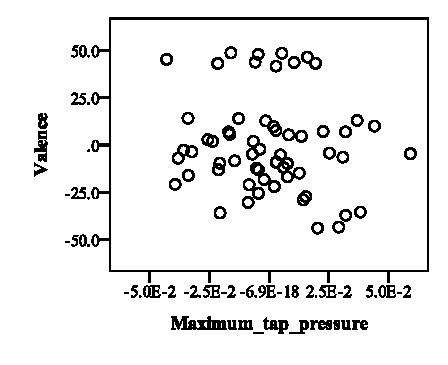
\includegraphics[width=\textwidth]{images/linearity/partialregression/valence/ValMaxMax.eps}
    \label{fig:valmaxmax}
  \end{subfigure}
  \quad
  \begin{subfigure}[b]{0.45\textwidth}
    \centering
    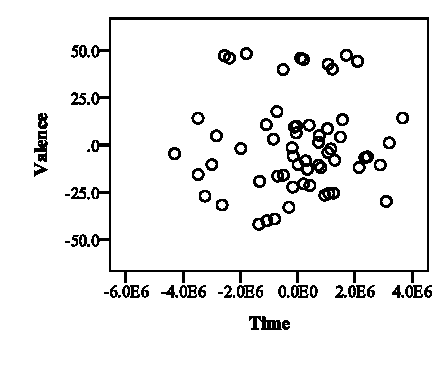
\includegraphics[width=\textwidth]{images/linearity/partialregression/valence/ValMaxTime.eps}
    \label{fig:valmaxtime}
  \end{subfigure}
  \caption{Partial regression plots with valence (dependent variable), maximum pressure and duration (independent variables). Note the approximate linearity.}
\end{figure}

\begin{figure}[ht]
  \centering
  \begin{subfigure}[b]{0.45\textwidth}
    \centering
    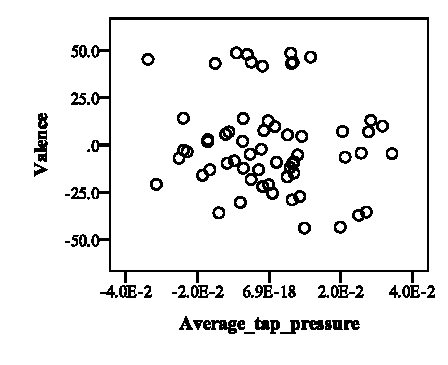
\includegraphics[width=\textwidth]{images/linearity/partialregression/valence/ValAvgAvg.eps}
    \label{fig:valavgavg}
  \end{subfigure}
  \quad
  \begin{subfigure}[b]{0.45\textwidth}
    \centering
    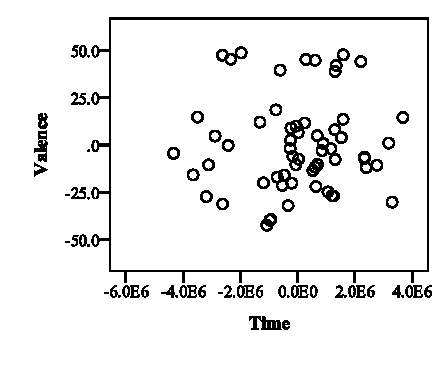
\includegraphics[width=\textwidth]{images/linearity/partialregression/valence/ValAvgTime.eps}
    \label{fig:valavgtime}
  \end{subfigure}
  \caption{Partial regression plots with valence (dependent variable), average pressure and duration (independent variables). Note the approximate linearity.}
\end{figure}